\PassOptionsToPackage{force}{filehook}

\documentclass{beamer}
\usecolortheme{wolverine}
\setbeamertemplate{footline}[frame number]
%\useoutertheme{split}
%\useinnertheme{rounded}
\usepackage{pgf,tikz}
\usetikzlibrary{positioning}
\usepackage{amsmath}
\usepackage{amsfonts}
\usepackage{graphicx} 
\usepackage{subcaption}
\usepackage{hyperref}
\usepackage{cancel}
\usepackage{wrapfig}
\usepackage{comment}
\hypersetup{
	colorlinks=true,
	linkcolor=blue,
	filecolor=magenta,      
	urlcolor=cyan,
}
\usepackage{color}
\usepackage{mathpazo}
\usepackage{enumitem}
\usepackage{hyperref}
\usepackage{multimedia}
\usepackage{graphicx}
%\usepackage[demo]{graphicx}
\usepackage{caption}
\usepackage{subcaption}
\usepackage{textcomp}
\usepackage{graphicx} 
\usepackage{booktabs}
\usepackage{cite}
\usepackage{hyperref}
\usepackage{multicol}
\usepackage{multirow,array}
\usepackage{amsmath}
\usepackage{mathrsfs}
\usepackage{amssymb}
\usepackage[utf8]{inputenc}
\usepackage{amsthm}
\newtheorem{thm}{Teorema}
\newtheorem{lem}[thm]{Lema}
\newtheorem{axiom}[thm]{Axioma}
\newtheorem{prop}[thm]{Proposici\'on}
\newtheorem{cor}[thm]{Corolario}
\theoremstyle{definition}
\newtheorem{defn}{Definici\'on}
\DeclareGraphicsExtensions{.pdf,.jpeg,.png,.eps}
%\usetheme{CambridgeUS}
\setbeamertemplate{navigation symbols}{}
\usepackage{pgf,tikz}
\usetikzlibrary{positioning}
\usepackage[spanish, activeacute]{babel} %Definir idioma español
\usepackage[utf8]{inputenc} %Codificacion utf-8
\usepackage{multirow}
\def\mydate{\leavevmode\hbox{\twodigits\day/\twodigits\month/\the\year}}
\def\twodigits#1{\ifnum#1<10 0\fi\the#1}

%   Esconder las soluciones
\newif\ifhideproofs
\hideproofstrue %uncomment to hide proofs

\ifhideproofs
\usepackage{environ}
\NewEnviron{hide}{}
\let\solucion\hide
\let\endsolucion\endhide
\fi

\def\mydate{\leavevmode\hbox{\twodigits\day/\twodigits\month/\the\year}}
\def\twodigits#1{\ifnum#1<10 0\fi\the#1}
\definecolor{rosee}{rgb}{0.7,0.05,0.25}
\usepackage[final]{pdfpages}

\title{Microeconom\'ia}
\subtitle{Minimizaci\'on de Costos. Corto y Largo Plazo. Funci\'on de Oferta - 2/2 \\ \mydate}
\author[Minimización costos 2/2]{Lara Sánchez Peña\footnote{Basado en las notas de Marcos Ariel Lissauer}}
\institute[]{UTDT}
\medskip
\date[UTDT 2021]{}
% - Either use conference name or its abbreviation.
% - Not really informative to the audience, more for people (including
%   yourself) who are reading the slides online

%\subject{}}
% This is only inserted into the PDF information catalog. Can be left
% out. 

% If you have a file called "university-logo-filename.xxx", where xxx
% is a graphic format that can be processed by latex or pdflatex,
% resp., then you can add a logo as follows:

% \pgfdeclareimage[height=0.5cm]{university-logo}{university-logo-filename}
% \logo{\pgfuseimage{university-logo}}

% Delete this, if you do not want the table of contents to pop up at
% the beginning of each subsection:
%\AtBeginSubsection[]
%{
  %\begin{frame}<beamer>{Outline}
    %\tableofcontents[currentsection,currentsubsection]
  %\end{frame}
%}

% Let's get started
\begin{document}
\begin{frame}
  \titlepage
\end{frame}

\begin{frame}{Objetivos}

\begin{itemize}
\item Relación entre las curvas de costos en el corto y largo plazo.
\item ¿Qué mide $\mu$ el multiplicador de Lagrange?
\item Oferta de la firma en el corto plazo, beneficios y excedente del productor.
\item Oferta de la firma en el largo plazo.
\item Oferta de la industria en el corto y largo plazo.
\item Material de repaso: Ver las slides de Eco 1 en el campus 5.3 + archivo de GeoGebra costos CP\&LP, 6.1 y 6.4.
\end{itemize}
    
\end{frame}

\begin{frame}{Relaci\'on entre costos de corto y largo plazo}
\begin{itemize}

%\item En el corto plazo alguno de los insumos se encuentra fijo, mientras que en el largo todos los factores se pueden elegir \'{o}ptimamente de forma tal de minimizar el costo de producci\'{o}n.
\item Queremos comparar el costo de corto plazo $C_s(y, k)$ con el costo de largo plazo $C(y)$ para producir una cantidad $y$ cualquiera.

%\item Imaginemos que el factor fijo es el tamaño de la planta, representado por $k$. La función de costos a corto plazo de la firma, dado que tiene una planta de $k$ metros cuadrados, es $C_s(y, k)$, donde $s$ representa el corto plazo.
%\item Para cada nivel de producción $y$, habrá algún tamaño de planta óptimo para lograr alcanzarlo; llamémoslo $k(y)$. $k(y)$ es la \textbf{demanda condicionada} del tamaño de la planta por parte de la firma por depende  del (está condicionada al) nivel de producción $y$.
%\item La función de costos a largo plazo es $C_s(y, k(y))$ que mide cuánto cuesta producir $y$, dado que la firma puede ajustar óptimamente el tamaño de su planta.

%\item La función de costos a largo plazo de la firma es igual a la función de costos a corto plazo cuando la firma puede elegir $k$  de manera óptima (de manera de minimizar los costos), es decir, $k=k(y)$:
%\begin{center}
%$C(y)=C_s(y, k(y))$
%\end{center}
%\item \textbf{¿Cuál es la relación entre los gráficos de las funciones de costos de corto y largo plazo?} Elijamos un nivel de producción $y^*$. Sea $k^* = k(y^*)$ el tamaño de planta óptima para ese nivel de producción $y^*$. 

%\item Para ese valor particular de $y$, $y^*$, vale que los costos de corto y largo plazo valen lo mismo. 

%\item Ahora bien, ¿cómo se comparan los costos de corto y largo plazo, si en el corto plazo se puede usar solamente $k^*$ pero se quiere producir una cantidad $y$ que no necesariamente sea igual a $y^*$?

%La función de costos a corto plazo correspondiente a una planta de tamaño $k^*$ será $C_s(y, k^*)$ y a largo plazo $C(y) = C_s(y, k(y))$, exactamente igual que antes.

\item El costo de corto plazo de producir $y$ será mayor o igual al costo de largo plazo. ¿Por qué? En el corto plazo $x_2=k^*$ y en el largo plazo $x_2$ se puede elegir de manera de minimizar los costos.

\item Consideremos la cantidad $y^*$ que se produce si se elige $x_2=k^*$ para minimizar el costo total. En ese caso los costos de CP y LP (y los costos medios) serán iguales. 
%\item Dado que una de sus elecciones a largo plazo siempre es elegir el tamaño de la planta $k^*$, su elección óptima para producir $y$ unidades debe tener unos costos que sean como máximo iguales a $C_s(y, k^*)$, lo que significa que debe ser capaz de obtener al menos los mismos resultados tanto si ajusta el tamaño de la planta como si lo mantiene fijo. Por lo tanto,
%\begin{center}
%$C(y)\leq C_s(y,k^*)$
%\end{center}
%cualquiera que sea el nivel de $y$.

%\item De hecho, dado un determinado nivel de $y$, a saber, %$y^*$, sabemos que:
%\begin{center}
%$C(y)= C_s(y,k^*)$
%\end{center}
%\item ¿Por qué? Porque en $y^*$ la elección óptima del %tamaño de la planta es $k^*$. Por lo tanto,
%en $y^*$ los costos a largo plazo y los costos a corto plazo son iguales.
%\item Notar que:
\begin{center}
$\scalebox{0.9}{$C(y)\leq C_s(y,k^*) \Leftrightarrow \frac{C(y)}{y}\leq \frac{C_s(y,k^*)}{y} \Leftrightarrow CMe(y)\leq CMe_s(y,k^*)$}$
\end{center}
\item Para otras cantidades $y$ la curva de costo medio a corto plazo siempre se encuentra por encima de la curva de costo medio a largo plazo y solamente la toca en un punto, $y^*$.
\end{itemize}
\end{frame}

\begin{frame}{Relaci\'on entre costos de corto y largo plazo}
	\begin{center}
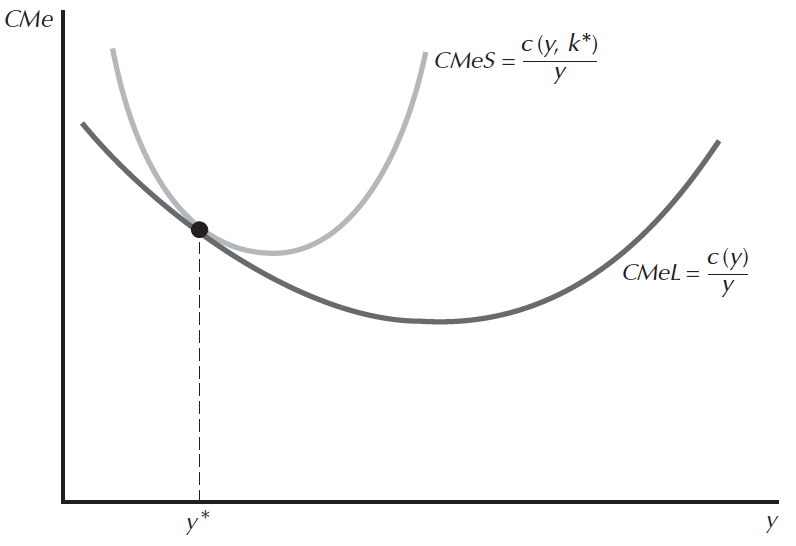
\includegraphics[width=3.8in]{figures4/shortlong1.png}
\end{center}
\end{frame}

\begin{frame}{¿Qué mide $\mu$?}\small
\begin{itemize}
%\item Relacionemos las soluciones de la maximización de beneficios y de la minimización de costos.
%\item  Las ecuaciones que caracterizan la soluci\'{o}n del problema de maximizaci\'{o}n de beneficios son:
%\begin{equation*}
%pPMg_{i}=w_{i}, \ \forall i
%\end{equation*}
\item Para la minimización de costos se plantea: \[\displaystyle\min_{x_1,x_2} w_1x_1+w_2x_2+\mu[y-f(x_1,x_2)]\]
\item Las condiciones que caracterizan la soluci\'{o}n del problema :
\begin{align}
\mu ^{c}\left( w_{1},w_{2},y\right) PMg_{1}\left( w_{1},w_{2},y\right)
=&w_{1},\label{eq1} \\
\mu ^{c}\left( w_{1},w_{2},y\right) PMg_{2}\left( w_{1},w_{2},y\right)
=&w_{2}, \label{eq2}\\
f\left( x_{1}^{c}\left( w_{1},w_{2},y\right) ,x_{2}^{c}\left(
w_{1},w_{2},y\right) \right) =&y \label{eq3}
\end{align}
%\end{itemize}
%\end{frame}

%\begin{frame}{Relaci\'on entre min. de costos y max. de beneficios}
%\begin{itemize}
%\item Si bien no es inmediato que las soluciones a los problemas vayan a coincidir (pues a\'{u}n no determinamos la cantidad a producir en la segunda etapa luego de minimizar los costos), podemos comenzar por interpretar $\mu ^{c}$.
\item Consideremos la función de costos $C(w_1,w_2,y)$ y derivemos respecto a $y$
\begin{equation}
\frac{\partial C\left( w_{1},w_{2},y\right) }{\partial y}=\frac{\partial
x_{1}^{c}}{\partial y}\color{rosee}w_{1}\color{black}+\frac{\partial x_{2}^{c}}{\partial y}\color{rosee}w_{2}\color{black} \label{eq4}
\end{equation}
\item Reemplacemos (\ref{eq1}) y (\ref{eq2}) en (\ref{eq4}),
\begin{equation}
\frac{\partial C\left( w_{1},w_{2},y\right) }{\partial y}=\frac{\partial x_{1}^{c}}{\partial y}\color{rosee}\mu ^{c}PMg_{1}\color{black}+\frac{\partial x_{2}^{c}}{\partial y}\color{rosee}\mu ^{c}PMg_{2}\color{black} \label{eq5}
\end{equation}
\end{itemize}
\end{frame}

\begin{frame}{¿Qué mide $\mu$?}\small
\begin{itemize}
\item Derivando (\ref{eq3}) respecto de $y$ a ambos lados:
\begin{equation}
PMg_{1}\frac{\partial x_{1}^{c}}{\partial y}+PMg_{2}\frac{\partial x_{2}^{c}}{\partial y}=1 \label{eq6}
\end{equation}
\item Notemos que el lado derecho de (\ref{eq5}) es igual a $\mu^c$ multiplicado por el lado izquierdo de (\ref{eq6})
\begin{equation*}
\frac{\partial C\left( w_{1},w_{2},y\right) }{\partial y}=\underset{=1}{%
\underbrace{\left[ \frac{\partial x_{1}^{c}}{\partial y}PMg_{1}+\frac{%
\partial x_{2}^{c}}{\partial y}PMg_{2}\right] }}\mu ^{c}
\end{equation*}
\item Es decir,
\begin{equation*}
\frac{\partial C\left( w_{1},w_{2},y\right) }{\partial y}=CMg(y)=\mu^{c} 
\end{equation*}
\item $\mu$ mide lo mínimo que aumenta la función de costo cuando se quiere producir un poco más de bien final. Es decir, $\mu$ es igual al costo marginal cuando se producen $y$ unidades del bien final.
\end{itemize}
\end{frame}

%\begin{frame}{¿Qué mide $\mu$?}
%\begin{itemize}
%\item Esto implica que en el \'{o}ptimo (cuando se eligen $x_1^c, x_2^c$ que minimizan costos) el valor del multiplicador de Lagrange, $\mu^c$ es igual al costo marginal. Es decir, es igual al aumento en el costo si la firma decidiera aumentar la producci\'{o}n. 
%\item Veremos a continuaci\'{o}n que debe ser cierto que el $CMg$ en el  \'{o}ptimo sea igual al precio del bien final. 

%\end{itemize}
%\end{frame}

\begin{frame}{Parte 2: Maximización de beneficios}\small
\begin{itemize}
\item \textbf{La soluci\'{o}n a la minimizaci\'{o}n de costos determina la mejor
manera de producir cualquier cantidad $y$}. El menor costo para producirla es $C(y)$, que depende de $w_1$ y $w_2$ porque la firma es tomadora de precios en esos mercados.
\item \textbf{En la segunda etapa, el objetivo es elegir la cantidad a producir la que maximiza los
beneficios de la firma}:
\begin{center}
$\max\limits_{y}py-C(y)$
\end{center}
\item Resolviendo este problema, la firma maximiza beneficios si iguala ingreso marginal ($p$, es constante porque la firma es tomadora de precios) al costo marginal:
\begin{align}
p=C'(y)=CMg(y) \label{eqmaxpi}
\end{align}
\item Para asegurarnos de que (\ref{eqmaxpi}) caracteriza un m\'{a}ximo debemos
verificar la \textbf{condici\'{o}n de segundo orden}, que en este caso es $C''(y)>0$. Es decir, la funci\'{o}n de costos debe ser convexa (ver slides 4 \S14).
\end{itemize}
\end{frame}

\begin{frame}{Oferta de una firma en el corto y largo plazo}
Para una tecnología como la de las slides 4 \S17 - \S22:
\begin{itemize}
\item En el \color{cyan} \textbf{corto plazo}\color{black}, una firma producirá $y>0$ si \begin{align*}
\pi_{\text{producir}}=py – CV(y) – F\geq& -F=\pi_{\text{no producir}}\\ p \geq & CMeV(y)\end{align*}

\item Por lo tanto, la firma ofrecerá cantidades $y>0$ en el \color{cyan} \textbf{corto plazo} \color{black} usando que $p=CMg(y)$ si $CMg(y)>CMeV(y)$.\footnote{En el corto plazo se dice que la firma \textbf{cierra} si no produce y en el largo plazo se dice que la firma \textbf{sale del mercado} si no produce.} 

\item En el \color{rosee} \textbf{largo plazo}\color{black}, una firma producirá $y>0$ si \begin{align*}\pi_{\text{producir}}=py – C(y)\geq& 0=\pi_{\text{salir del mercado}}\\  p \geq & CMe(y)\end{align*}

\item Por lo tanto, la firma ofrecerá cantidades $y>0$ en el \color{rosee} \textbf{largo plazo} \color{black} usando que $p=CMg(y)$ si $CMg(y)>CMe(y)$. 

%\item Para que se cumpla la CSO, la funci\'{o}n de costos tiene que ser estrictamente convexa, lo que implica que la funci\'{o}n de producci\'{o}n es estrictamente c\'{o}ncava en $y$. Recordemos que esta es la misma condición que pedíamos cuando vimos el problema de maximización de beneficios, pedíamos que $f(x_1,x_2)$ fuera estrictamente convexa en $(x_1,x_2)$.
%\item Llamemos $y^{\ast}$ a la soluci\'{o}n del problema de maximizaci\'{o}n de beneficios. Si en $y^{\ast}$ la tecnolog\'{\i}a tiene rendimientos no crecientes a escala, entonces:
%\begin{center}
%$CMg(y^{\ast })\geq CMe(y^{\ast })$
%\end{center}
%\item Lo que implica que los beneficios de la firma son no negativos:
%\begin{center}
%$py^{\ast }-C(y^{\ast })=y^{\ast}(CMg(y^{\ast })-%CMe(y^{\ast }))\geq 0$
%\end{center}
\end{itemize}
\end{frame}

\begin{frame}{Oferta de una firma en el corto y largo plazo}
\begin{columns}\hspace{-0.5em}
\begin{column}[t]{0.48\textwidth}
\begin{center}
\textbf{Corto plazo} \\
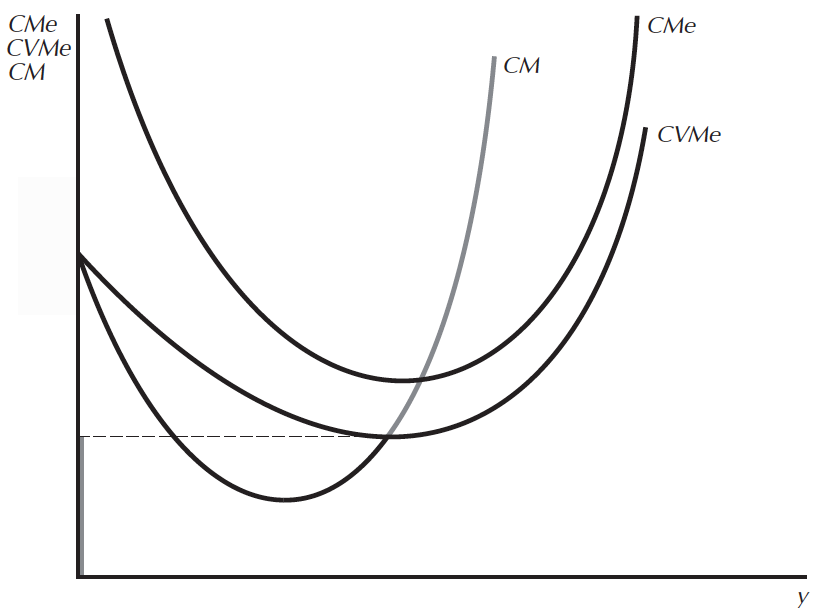
\includegraphics[scale=0.37]{figures4/oferta.png} 
\end{center}  \small Notemos que la firma ofrece cantidades $y$ -que se calculan usando $p=CMg(y)$- si $p \geq CMeV_{\text{mín}}$. Es decir, el bien $y$ es un bien ordinario.
\end{column}
\begin{column}[t]{0.48\textwidth}
\begin{center}
\textbf{Largo plazo} \\
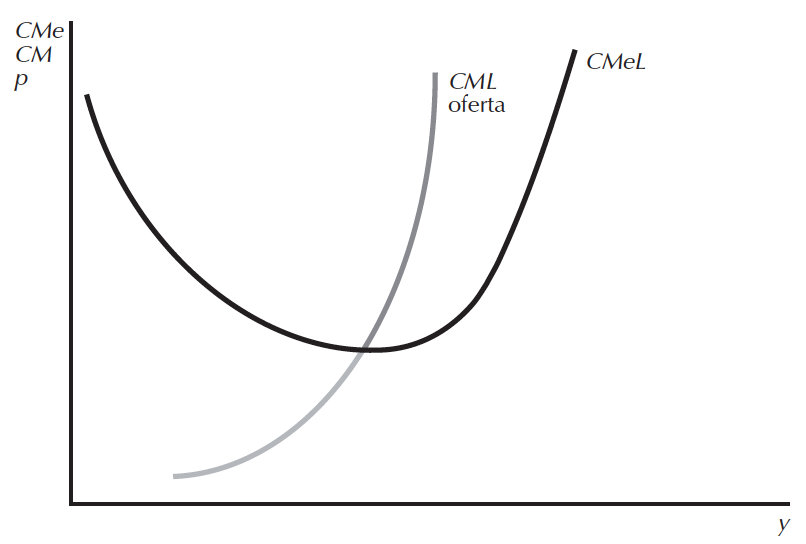
\includegraphics[scale=0.4]{figures4/cmgLP.png}
\end{center}  \small Notemos que la firma ofrece cantidades $y$ -que se calculan usando $p=CMg(y)$- si $p \geq CMe_{\text{mín}}$. Es decir, el bien $y$ es un bien ordinario.
\end{column}
\end{columns}
\end{frame}

\begin{frame}{Oferta de LP de una firma si la tecnología tiene CRS}
\begin{itemize}
\item En el largo plazo, si $f(tx_1,tx_2)=tf(x_1,x_2)$ vale que $C(y)=cy$. El beneficio de la firma es:
\begin{center}
$\pi =(p-c)y$
\end{center}
\item Vimos que si $p>c$ el problema no tiene soluci\'{o}n porque la firma querría ofrecer $y\rightarrow
\infty$. Si $p<c$, el problema la firma no querría producir $y=0$.
\item Si $p=c$, el problema la firma está indiferente en producir $y\in [0,+\infty)$.


\item La curva de oferta a largo es una recta horizontal. ¿Por qué? Como $C(y)=cy$, entonces $CMe(y)=CMg(y)=c$, por lo tanto la curva de costo marginal es igual a la curva de costo medio en el largo plazo. %Esto ocurre porque, cuando los costos medios son constantes, la curva de costo marginal coincide con la curva de costo medio a largo plazo.

\item Por lo tanto, la curva de oferta a
largo plazo es una recta horizontal en $p=c$.

\end{itemize}
\end{frame}

\begin{frame}{Oferta de LP de una firma si la tecnología tiene CRS}
\begin{center}
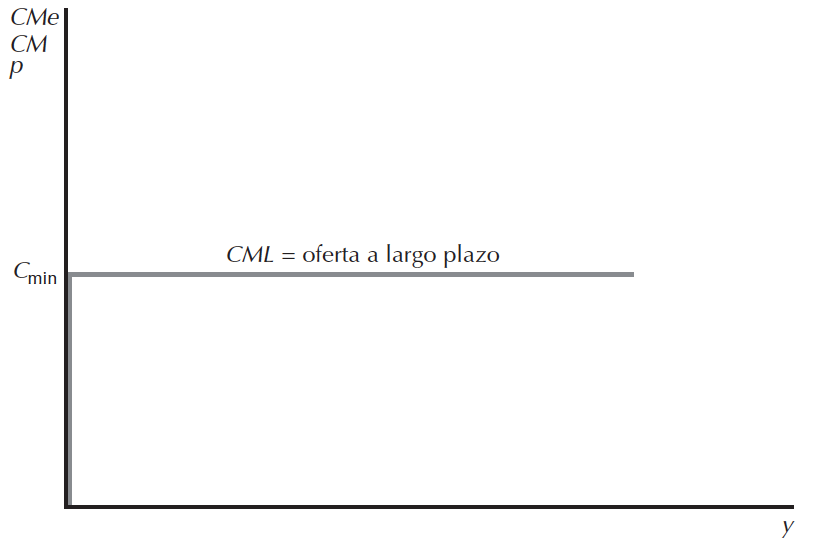
\includegraphics[width=3.2in]{figures4/RCSLP.png}
\end{center}

\medskip

\textbf{Nota:} Si la tecnología que utiliza una firma tuviera $DRS$ entonces la oferta tendría pendiente positiva. 
\end{frame}

\begin{frame}{Beneficios vistos gráficamente}
\begin{columns}
    \begin{column}[t]{0.52\textwidth}
\small
\begin{center}
 Para ver gráficamente los beneficios $\pi=IT-CT$:
\begin{enumerate}
    \item Los ingresos totales $IT$ son: $IT=p\cdot y=CMg(y)\cdot y$. Los $IT$ se miden con el \'area del rectángulo que tiene base $y$ y altura $CMg(y)$.
    \item Los costos totales $CT$ son: $CT=CMe(y)\cdot y$. Los $CT$ se miden con el \'area del rectángulo que tiene base $y$ y altura $CMe(y)$.
\end{enumerate} 
\end{center}
\end{column}
\begin{column}[t]{0.46\textwidth}
\begin{center}
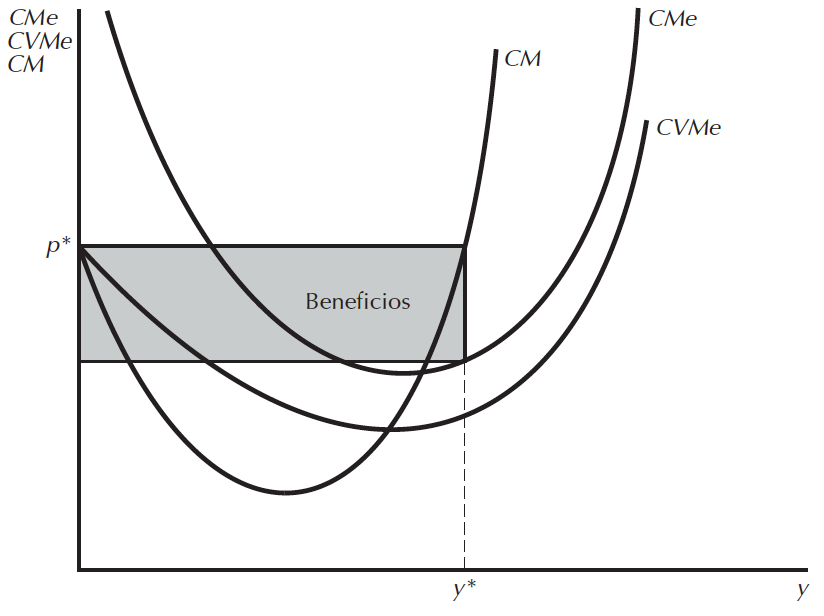
\includegraphics[scale=0.38]{figures4/beneficios.png}

 \small Los beneficios, se miden con la diferencia entre ambas \'areas
\[\pi =(CMg(y)-CMe(y))\cdot y\]
\end{center} 
\end{column}
\end{columns}
\end{frame}

\begin{frame}{Beneficios vistos gráficamente}
    \begin{itemize}
        \item La empresa A tiene beneficios iguales a cero.
        \item La empresa B tiene beneficios mayores a cero.
        \item La empresa C tiene beneficios menores a cero. En el largo plazo la firma no produciría esa cantidad. En el corto plazo la firma produciría esa cantidad si $\pi_{\text{producir}}>\pi_{\text{no producir}}=-F$.
    \end{itemize}
\begin{center}
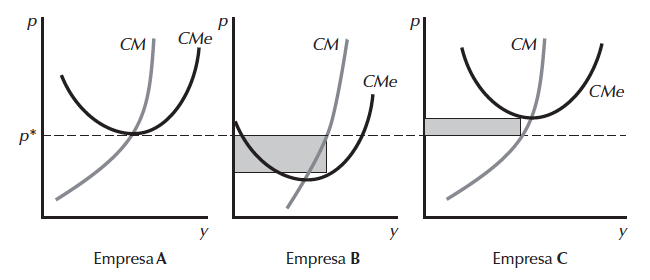
\includegraphics[width=3.8in]{figures5/industry_profits.png}
\end{center}
\end{frame}

\begin{frame}{Excedente del productor}
\begin{itemize}
%Es el ingreso extra que la firma obtiene por operar en una econom\'{i}a de mercado en donde todas sus unidades se venden al mismo precio.
\item El \textbf{excedente del productor} (EP) es otra medida de bienestar de la firma. 
\item En el \textbf{largo plazo}, $EP=\pi$
\item En el \textbf{corto plazo},
\begin{enumerate}[label=\textbf{(\Alph*)}]
    \item $EP=IT-CV$, ingresos menos
los costos variables.
    \item $EP=\pi+F$, beneficios más los costos fijos
    \end{enumerate}
    \item Gráficamente $EP=(p-CMV(y))y$ Es decir que es la diferencia del \'area del rectángulo de:
\begin{itemize}
    \item los \textbf{ingresos totales}: $p\cdot y=CMg(y)\cdot y$
    \item los \textbf{costos variables}: $CMe(y)\cdot y$
\end{itemize}

\begin{enumerate}[label=\textbf{(\Alph*)}]
\setcounter{enumi}{2}
    \item Es el \'area por arriba del costo marginal para el rango de precios  $[p_{\text{min}},p]$. Donde $p$ es el precio de mercado y $p_{\text{min}}$ es el mínimo precio para el que la firma vende.
%    \item $EP=\displaystyle\int\limits_{p_{0}}^{p}y\left( p\right) dp$ donde $p_{0}=CMeV_{min}$. Noten que la integral definida sobre el eje vertical.
\end{enumerate}

\end{itemize}
\end{frame}


\begin{frame}{Variaci\'on en el excedente del productor}

\begin{columns}
    \begin{column}[t]{0.48\textwidth}
    \begin{itemize}[leftmargin=*]\small
       \item Supongamos que el precio cambia $p^*$ a $p^{'}$. Por ejemplo, $p^*<p^{'}$, es decir, el precio aumenta. La variación en el $EP$ mide cuánto cambia el bienestar del productor.
        
\item Notemos que la variación en el excedente del productor es igual que la variación de los beneficios en la misma situación ya que los costos fijos
no varían. 

\end{itemize}
    \end{column}
    \begin{column}[t]{0.48\textwidth}
       \begin{center}
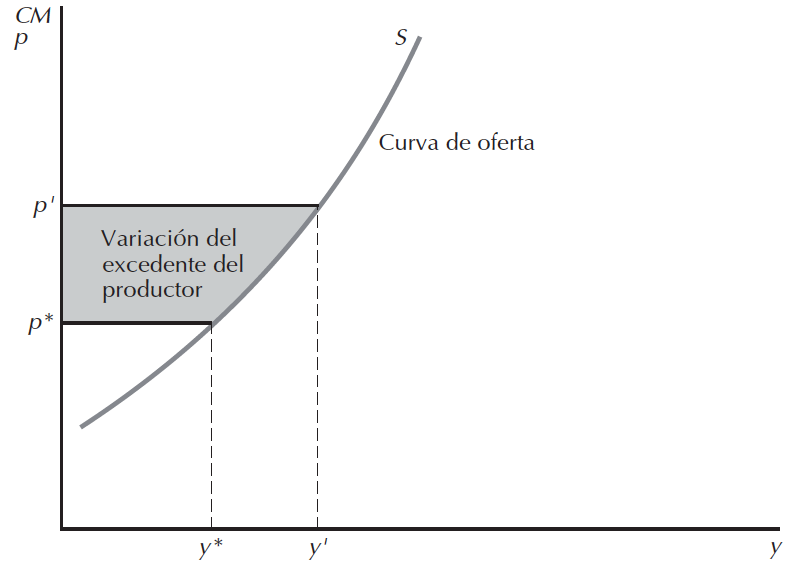
\includegraphics[scale=0.39]{figures4/varEP.png}
\end{center} 
    \end{column}
\end{columns}

\medskip
\small
En este caso como el precio del bien final la variación en el excedente del productor, $\Delta EP$, es positivo porque los beneficios aumentan luego del aumento en el precio al que se vende cada unidad.

\end{frame}

\begin{frame}{Oferta de una firma: Corto vs largo plazo}
\small
\begin{columns}
\begin{column}[t]{0.46\textwidth}
\begin{itemize}[leftmargin=*]
\item Consideremos el precio $p^*$ que en el largo plazo maximiza los beneficios si se produce la cantidad $y^*$.

\item Imaginemos que en el corto plazo (para este gráfico) se cuenta con la cantidad $x_2=k^*$ que, vendiendo a precio $p^*$, se maximizan los beneficios produciendo $y^*$.

\item Por lo tanto, para la cantidad $y^*$ las curvas de oferta de corto plazo y de largo plazo se intersecan en $(y^*,p^*)$ si el factor fijo de corto plazo es $x_2=k^*$.
\end{itemize}
\end{column}
 \begin{column}[t]{0.52\textwidth}
    \begin{center}
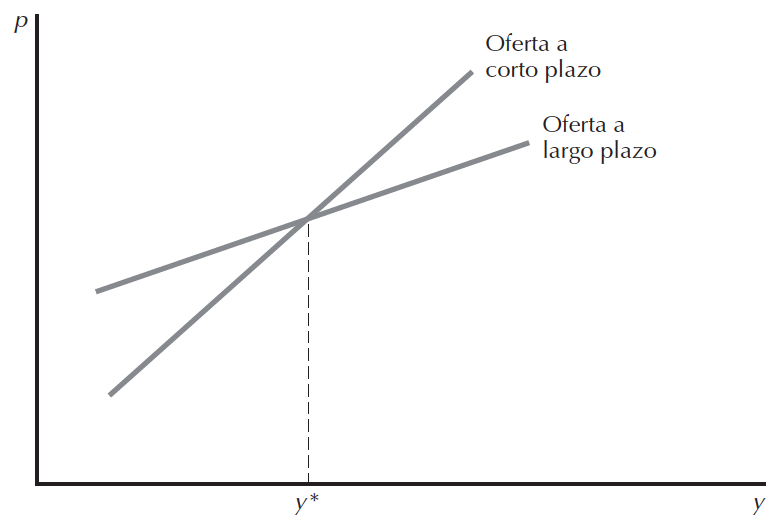
\includegraphics[scale=0.4]{figures4/LP.png}
\begin{itemize}[leftmargin=*]
    \item 
Para otros valores de $p\neq p^*$, en el largo plazo la firma puede elegir ambos insumos, lo que implica que la cantidad ofrecida a largo plazo puede potencialmente cambiar más ante un cambio en el precio precio (más elástica) que la de corto plazo. %Esto ocurre porque la cantidad ofrecida puede potencialmente cambiar más ante un cambio en el precio.
\end{itemize}
\end{center}
    \end{column}
\end{columns}
\end{frame}


\begin{frame}{Oferta agregada (de la industria) con libre entrada y salida}
    \begin{itemize}
        \item En el \textbf{largo plazo}, las firmas pueden elegir:
        \begin{itemize}
            \item las cantidades de todos sus insumos,
            \item si entran o salen del mercado.
        \end{itemize}
        
        \item Decimos que hay \textbf{libre entrada y salida} de firmas.
       % \item Si una firma pierde dinero en el largo plazo, puede salir del mercado. De la misma manera, si las firmas se encuentran obteniendo beneficios positivos en el largo plazo, esperaremos que más firmas ingresen al mercado, dado que todas las firmas tienen acceso a la tecnología de producción.

       \item A priori cada una de las firmas podría tener su tecnología de producción.
       \item Concentrémonos en dos casos particulares donde \textbf{todas las firmas tienen la misma tecnología} con:
       \begin{itemize}
           \item \textbf{CRS}: En este caso, la oferta agregada es horizontal como vimos en la slide \S11. En ese mercado se vende a precio $p=c$ y no queda determinada cuántas firmas venden.
           \item \textbf{DRS}: Aquí hay que obtener la demanda agregada que se determina de a tramos (cuanto mayor sea $p$ mayor cantidad de firmas quiere entrar porque también aumentan los costos medios de producción (al entrar más firmas produce cada una menos y a un costo medio menor).
       \end{itemize}
    \end{itemize}
\end{frame}


\begin{frame}{Oferta agregada de firmas con la misma tecnología (DRS)}
\small Una vez que encontramos la oferta de cada firma podemos encontrar la oferta de la industria sumando las ofertas individuales de las $n$ firmas: $S(p) = \sum_{i=1}^{n}s_{i}(p)$
    
 \medskip Para determinar la demanda agregada con una tecnología que tiene DRS  hay que graficar las ofertas de $n=1$, $n=2$, $\cdots$ firmas y ver a partir de qué cantidades querrían ofrecer quisiera entrar una firma más en el margen. Notar que en el gráfico las demandas con líneas punteadas se grafican a partir del mismo valor de $p$ que es el $CMe_{\text{mín}}$.


    \begin{center}
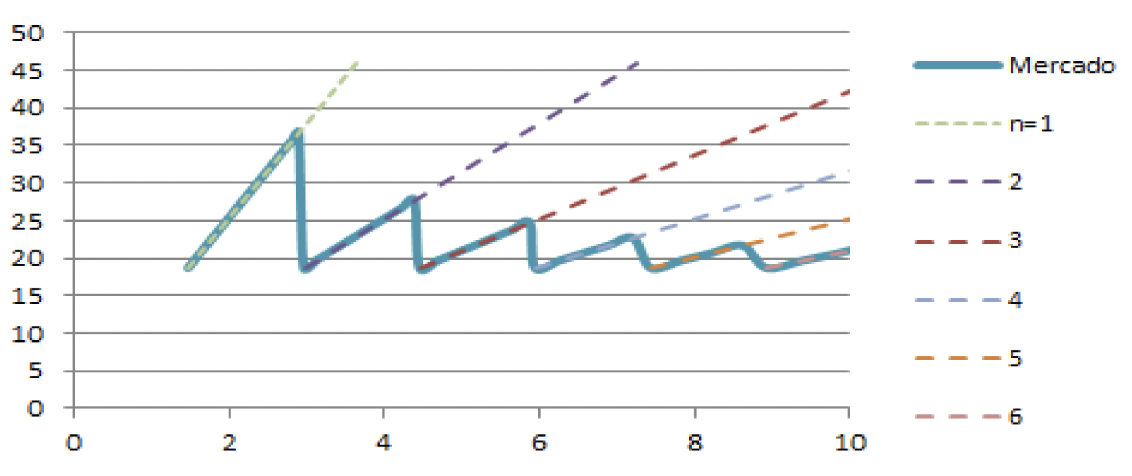
\includegraphics[scale=0.5]{figures5/ofertaagregadaDRS.png}
\end{center}
\end{frame}

\begin{frame}{Equilibrio de largo plazo}\small
\begin{itemize}[leftmargin=*]
 \item   Cuando hay libre entrada y salida de firmas, porque las firmas pueden decidir entrar o salir, un \textbf{equilibrio de largo plazo} se compondrá de tres cosas:
    \begin{enumerate}
    \item precio $p^*$ de equilibrio
    \item cantidad $y^*$ de equilibrio
    \item cantidad $n^*$ de firmas que venden en equilibrio.
    \end{enumerate}
    \item Suponiendo que todas las firmas tienen la misma tecnología, $S(p) = \sum_{i=1}^{n}s_{i}(p)=ns_1(p)$ 
    la idea sería encontrar $(p,^*,y^*,n^*)$ que cumplan que:    
\begin{align*}
    ns_1(p)=D(p) \qquad \text{ y además } \qquad \pi(p)=0
\end{align*}
\item La \textbf{primera condición} dice que oferta de mercado es igual a demanda de mercado. 
\item La \textbf{segunda condición} dice que las firmas tienen que estar \textbf{indiferentes entre producir y no producir}. ¿Por qué? Porque si $\pi(p)>0$ como cada firma obtiene $\pi(p)$ beneficios más firmas querrían empezar a producir. Si $\pi(p)<0$ habría firmas que querrían dejar de producir.
    
    \end{itemize}
\end{frame}

\begin{frame}{Equilibrio de largo plazo: ejercicios}
\small
Encuentre el \textbf{equilibrio de largo plazo} para ambos ejercicios suponiendo que $w_1=1$, $w_2=31$ y $P(y)=\frac{8}{y}$.

\begin{enumerate}
    \item Para $f(x_1,x_2)=\min\{2x_1,x_2\}$ muestre que
    \begin{itemize} \color{gray}
        \item $C(y)=\left(\frac{w_1}{2}+w_2\right)\cdot y$ es decir $C(y)=31.5y$.
        \item la oferta de cada firma es $p=p^*=31.5$.  
        \item $\pi^*=0$ sin tener que pedir una condición extra.
        \item $y^*=\frac{16}{63}$.
        \item Note que la cantidad de firmas queda indeterminada.
    \end{itemize}
    \item Para $f(x_1,x_2)=\min\{x_1-4,x_2\}^{\frac{1}{2}}$ muestre que
    \begin{itemize} \color{gray}
        \item $C(y)=\left(w_1+w_2\right)\cdot y^2+w_1\cdot 4$ es decir $C(y)=32y^2+4$.
        \item la oferta de cada firma es $p=64y$. O sea, $y=\frac{p}{64}$.
        \item la oferta agregada inversa es $y^{\text{ag}}=n\frac{p}{64}$ o sea la oferta agregada es $p=\frac{64}{n}y$. 
        \item Igualando oferta y demanda de mercado, $y^*=\sqrt{\frac{n}{8}}$ y $p^*=\sqrt{\frac{8}{n}}$.
        \item $\pi^*=8-4n-4$. O sea que $\pi^*=0$ si $n^*=1$.
        \item Entonces $y^*=\frac{1}{2}$, $p^*=\sqrt{8}$.
    \end{itemize}
\end{enumerate}
\end{frame}





\end{document}